% =================================================================
% Parameter-Efficient Variational Quantum Circuits:
% A Systematic Comparison of FC, Residual, and Transformer Architectures
% =================================================================
\documentclass[twocolumn,prl,amsmath,amssymb,superscriptaddress]{revtex4-2}
% Alternative: \documentclass[conference]{IEEEtran}

\usepackage{graphicx}
\usepackage{booktabs}
\usepackage{amsmath,amssymb}
\usepackage{hyperref}
\usepackage{xcolor}
\usepackage{multirow}
\usepackage{subcaption}

% Shorthand
\newcommand{\R}{\mathbb{R}}
\newcommand{\KL}{D_{\mathrm{KL}}}
\newcommand{\QT}{\text{QT}}
\newcommand{\FQT}{\text{FQT}}

\begin{document}

\title{Parameter-Efficient Variational Quantum Circuits:\\
A Systematic Comparison of Fully-Connected, Residual,\\
and Transformer Architectures}

\author{Chi-Sheng Chen}
% \affiliation{...}

\date{\today}

\begin{abstract}
Variational quantum circuits (VQCs) are a leading approach to quantum machine
learning on near-term devices, yet it remains unclear which circuit
architecture yields the best accuracy--parameter trade-off on classical
tabular data.  We present a systematic empirical comparison of four VQC
families---multi-layer fully-connected (FC-VQC), residual (ResNet-VQC),
hybrid quantum--classical transformer (QT), and fully quantum transformer
(FQT)---across five regression and classification benchmarks.
Our key findings are:
\textbf{(i)}~FC-VQCs achieve competitive or superior regression accuracy to
gradient-boosted trees with \emph{orders-of-magnitude fewer parameters}
(e.g.\ $R^2{=}0.889$ on Boston Housing with only 720 parameters);
\textbf{(ii)}~quantum self-attention provides no consistent benefit on
small-scale tabular data---ablations show that removing attention can
\emph{improve} performance;
\textbf{(iii)}~expressibility saturates at circuit depth~${\approx}\,3$,
explaining why shallow VQCs already cover the Hilbert space effectively;
\textbf{(iv)}~LayerNorm on the fully quantum transformer improves
classification accuracy, suggesting normalization is important when all
operations are quantum.
% TODO: Add noise-robustness finding after experiments complete.
These results provide practical architectural guidance for deploying VQCs on
near-term quantum hardware.
\end{abstract}

\maketitle

% =================================================================
\section{Introduction}
\label{sec:intro}
% Introduction — repositioned as systematic empirical comparison

Variational quantum circuits (VQCs) have emerged as one of the most promising
paradigms for quantum machine learning on near-term intermediate-scale quantum
(NISQ) devices~\cite{cerezo2021variational,benedetti2019parameterized}.
By parameterizing quantum gates and optimizing them via classical gradient
methods, VQCs combine the expressiveness of quantum Hilbert space with the
practicality of hybrid quantum--classical training loops.

Despite growing interest, the design space of VQC architectures remains
poorly understood.  Classical deep learning has benefited enormously from
systematic architectural comparisons---fully-connected networks versus
convolutional networks versus transformers---which yielded clear guidelines on
when each topology excels.  No analogous study exists for VQCs.  Most prior
work proposes a single new circuit ansatz and evaluates it on one or two
benchmarks, making it difficult to draw general conclusions.

In this work, we address this gap with a \emph{systematic empirical
comparison} of four VQC architecture families on tabular regression and
classification tasks:

\begin{enumerate}
  \item \textbf{Multi-layer fully-connected VQC (FC-VQC)} ---
    cascaded VQC blocks with all-to-all inter-block connectivity
    and configurable qubit layouts (e.g.\ $16 \to 4 \to 1$).
  \item \textbf{Residual VQC (ResNet-VQC)} ---
    VQC layers augmented with classical residual (skip) connections,
    inspired by He et al.~\cite{he2016deep}.
  \item \textbf{Quantum Transformer VQC (QT)} ---
    a hybrid architecture where classical self-attention operates on
    quantum-encoded features (Route~A).
  \item \textbf{Fully Quantum Transformer VQC (FQT)} ---
    an architecture where both the attention mechanism and the
    feed-forward network are implemented as parameterized quantum
    circuits (Route~B).
\end{enumerate}

All architectures are evaluated on five datasets (three regression, two
classification) against strong classical baselines including XGBoost,
CatBoost, and parameter-matched MLPs.  We further conduct ablation studies
on the transformer components and measure circuit expressibility using the
Sim et al.~\cite{sim2019expressibility} KL-divergence metric.

Our main contributions are:
\begin{itemize}
  \item A unified experimental framework enabling fair, controlled comparison
    across VQC architectures on identical data splits, training protocols,
    and evaluation metrics.
  \item Evidence that \textbf{FC-VQCs are the most parameter-efficient}
    architecture, achieving regression accuracy competitive with
    gradient-boosted trees using ${\sim}$700 parameters versus
    ${\sim}$13{,}000 for equivalently accurate MLPs.
  \item A \textbf{negative result on quantum attention}: self-attention
    does not consistently help on small tabular data, and removing it can
    improve performance---an important finding for practitioners.
  \item Practical guidance: expressibility saturates at depth~${\approx}\,3$,
    LayerNorm benefits fully quantum architectures on classification, and
    residual connections offer a reliable middle ground between FC-VQC and
    transformer complexity.
\end{itemize}


% =================================================================
\section{Related Work}
\label{sec:related}
% TODO: Draft related work
% Key areas:
% - VQC / PQC literature (Cerezo et al., Benedetti et al.)
% - Expressibility metrics (Sim et al. 2019)
% - Quantum transformers / quantum attention (prior work)
% - Residual connections in quantum circuits
% - Barren plateaus and trainability


% =================================================================
\section{Methods}
\label{sec:methods}
% Methods

We compare four VQC architecture families, all built on the
\texttt{StronglyEntanglingLayers} ansatz from PennyLane as the base
quantum circuit block.

\subsection{Multi-Layer Fully-Connected VQC (FC-VQC)}

The FC-VQC cascades multiple VQC blocks with decreasing qubit counts,
connected via classical fully-connected (dense) layers.  For example,
the notation $16\mathrm{t}4\mathrm{t}1$ denotes a three-block architecture
mapping 16~qubits $\to$ 4~qubits $\to$ 1~qubit, with each block consisting
of \texttt{StronglyEntanglingLayers} at a fixed depth $d$ (typically~3).

Two inter-block connectivity modes are supported:
\begin{itemize}
  \item \textbf{Type~4 (fully-connected):} Each qubit measurement from
    block $\ell$ is connected to all angle-encoding inputs of block
    $\ell{+}1$ via a learned linear projection.
  \item \textbf{Type~3 (circular-shift):} A fixed permutation maps
    block $\ell$ outputs to block $\ell{+}1$ inputs, reducing parameters.
\end{itemize}

\subsection{Residual VQC (ResNet-VQC)}

ResNet-VQC augments the FC-VQC topology with classical residual connections.
When the qubit count is preserved between adjacent blocks ($n_\ell = n_{\ell+1}$),
a skip connection adds the input measurements to the output:
\begin{equation}
  \mathbf{z}_{\ell+1} = \mathrm{VQC}_{\ell+1}(\mathbf{z}_\ell) + \mathbf{z}_\ell.
\end{equation}
When dimensions differ, a learned linear projection is applied to the skip
path.  This mirrors classical ResNets~\cite{he2016deep} and is motivated by
the same goal: easing gradient flow through deep stacks of nonlinear blocks.

\subsection{Quantum Transformer VQC (QT --- Route A)}

QT implements a hybrid quantum--classical transformer block.  The input
features are first encoded into a VQC, whose measurement outputs serve as
token embeddings.  A \emph{classical} multi-head self-attention layer
operates on these embeddings, followed by a VQC-based feed-forward network:
\begin{equation}
  \mathbf{h} = \mathrm{Attention}(\mathrm{VQC}_{\mathrm{enc}}(\mathbf{x}))
  + \mathrm{VQC}_{\mathrm{enc}}(\mathbf{x}),
\end{equation}
\begin{equation}
  \mathbf{y} = \mathrm{VQC}_{\mathrm{ffn}}(\mathrm{LayerNorm}(\mathbf{h}))
  + \mathbf{h}.
\end{equation}
This route uses classical attention but quantum encoding and feed-forward
processing.

\subsection{Fully Quantum Transformer VQC (FQT --- Route B)}

FQT replaces the classical attention with a parameterized quantum circuit
that computes query--key interactions via entangling gates.  Both the
attention mechanism and the feed-forward network are implemented as VQCs,
making the entire transformer block quantum (except for measurement and
re-encoding).

We also study a \textbf{+LayerNorm} variant that applies classical
LayerNorm to the FQT outputs before the next layer, which our ablation
shows is important for classification performance.

\subsection{Noise Model}
\label{sec:noise-model}

To assess near-term hardware viability, we inject single-qubit depolarizing
noise after every layer of \texttt{StronglyEntanglingLayers}:
\begin{equation}
  \mathcal{E}(\rho) = (1 - p_d)\,\rho + \frac{p_d}{3}(X\rho X + Y\rho Y + Z\rho Z),
\end{equation}
where $p_d \in \{0.001, 0.005, 0.01, 0.05\}$ controls the noise strength.
% TODO: Expand after noise experiments are complete.


% =================================================================
\section{Experimental Setup}
\label{sec:setup}
% Experimental Setup

\subsection{Datasets}

We evaluate on five tabular benchmarks spanning regression and classification:

\begin{table}[h]
\centering
\small
\begin{tabular}{llrrr}
\toprule
Dataset & Task & $n$ & Features & Target \\
\midrule
Boston Housing & regression & 506 & 13 & MEDV \\
CA Housing & regression & 20{,}640 & 8 & MedHouseVal \\
Concrete & regression & 1{,}030 & 8 & strength \\
Wine (Red) & classification & 1{,}599 & 11 & quality \\
Wine (R+W) & classification & 6{,}497 & 12 & quality \\
\bottomrule
\end{tabular}
\caption{Dataset summary.}
\label{tab:datasets}
\end{table}

Features are standardized to zero mean and unit variance.  Regression targets
are also standardized; predictions are inverse-transformed for evaluation.
The top and bottom 4\% of regression targets are clipped to reduce outlier
sensitivity.  Data is split into 70\% train / 15\% validation / 15\% test
with a fixed random seed for reproducibility.

\subsection{Baselines}

\textbf{Classical ML:} Ridge regression, kernel ridge regression (RBF),
SVR/SVC (RBF), linear/logistic regression, XGBoost, CatBoost.  Boosting
methods use default hyperparameters.

\textbf{Parameter-matched MLP:} A classical MLP whose hidden layer sizes
are chosen so that the total parameter count matches the median quantum
model (${\sim}$200--220 parameters).  This controls for the possibility
that quantum models benefit simply from having more parameters than a
trivially small network.

\subsection{Training Protocol}

All quantum and MLP models are trained with Adam (lr$\,{=}\,0.005$, no
weight decay) for 10{,}000 epochs with full-batch gradient descent.
Best-model checkpointing selects the epoch with lowest validation loss.
Gradient norms are clipped at 1.0 to prevent divergence.

\subsection{Evaluation Metrics}

Regression: $R^2$ (coefficient of determination), RMSE, MAE.
Classification: accuracy, macro-averaged F1 score.
All metrics are reported on the held-out test set using the best-validation
checkpoint.


% =================================================================
\section{Results}
\label{sec:results}
% Results section — narrative follows the repositioned framing

% =================================================================
% Auto-generated by summarize_results.py
% =================================================================

% Main regression comparison (test R²)
\begin{table}[t]
\centering
\caption{Test $R^2$ on regression datasets. Best value per column in \textbf{bold}. MLP$_{\text{PM}}$ is parameter-matched to the median quantum model.}
\label{tab:main-regression}
\small
\begin{tabular}{lrrrr}
\toprule
Model & Boston & CA Housing & Concrete & \#params \\
\midrule
CatBoost & 0.861 & \textbf{0.857} & \textbf{0.933} & -- \\
KRR (RBF) & 0.671 & 0.783 & 0.779 & -- \\
Linear & 0.666 & 0.644 & 0.604 & -- \\
Ridge & 0.666 & 0.644 & 0.605 & -- \\
SVR (RBF) & 0.548 & 0.788 & 0.608 & -- \\
XGBoost & 0.856 & 0.853 & 0.904 & -- \\
\midrule
MLP$_{\text{PM}}$ & 0.769 & 0.793 & 0.843 & 218 \\
\midrule
FullQT ($L2$, $K3$) & 0.799 & 0.786 & 0.792 & 855 \\
FullQT ($L2$, $K3$), $H{=}2$ & 0.626 & 0.811 & 0.797 & 2,025 \\
FullQT ($L2$, $K3$), $H{=}3$ & 0.808 & 0.806 & 0.757 & 2,745 \\
FC-VQC_15t5t1 ($L3$, $K3$) & \textbf{0.889} & -- & -- & 720 \\
FC-VQC_16t4t1 ($L3$, $K3$) & 0.811 & -- & -- & -- \\
FC-VQC_8t3t1 ($L3$, $K3$) & -- & 0.752 & 0.756 & 486 \\
QT ($L2$, $K3$) & 0.781 & 0.807 & 0.838 & 1,380 \\
QT ($L2$, $K3$), $H{=}2$ & 0.763 & 0.813 & 0.869 & 3,090 \\
QT ($L2$, $K3$), $H{=}3$ & 0.834 & 0.814 & 0.837 & 4,350 \\
ResNet-VQC_15t5t1 ($L3$, $K3$) & 0.831 & -- & -- & 720 \\
ResNet-VQC ($L3$, $K3$) & -- & 0.785 & 0.858 & 486 \\
\bottomrule
\end{tabular}
\end{table}

% Main classification comparison (test Accuracy / F1)
\begin{table}[t]
\centering
\caption{Test Accuracy and macro-F1 on classification datasets. Best value per column in \textbf{bold}.}
\label{tab:main-classification}
\small
\begin{tabular}{lrrrrr}
\toprule
Model & \multicolumn{2}{c}{Wine (Red)} & \multicolumn{2}{c}{Wine (R+W)} & \#params \\
\cmidrule(lr){2-3}\cmidrule(lr){4-5}
 & Acc & F1 & Acc & F1 & \\
\midrule
CatBoost & 0.667 & 0.330 & 0.675 & 0.422 & -- \\
LogReg & 0.608 & 0.275 & 0.557 & 0.270 & -- \\
SVC (RBF) & 0.604 & 0.271 & 0.592 & 0.271 & -- \\
XGBoost & \textbf{0.671} & \textbf{0.333} & \textbf{0.695} & \textbf{0.478} & -- \\
\midrule
MLP$_{\text{PM}}$ & 0.604 & 0.283 & 0.573 & 0.287 & 198 \\
\midrule
FullQT ($L2$, $K3$) & 0.608 & 0.293 & 0.592 & 0.294 & 678 \\
FullQT ($L2$, $K3$), $H{=}2$ & 0.583 & 0.284 & 0.581 & 0.280 & 1,470 \\
FullQT ($L2$, $K3$), $H{=}3$ & 0.600 & 0.282 & 0.585 & 0.286 & 1,974 \\
FC-VQC_12t8t6 ($L3$, $K3$) & 0.596 & 0.265 & 0.585 & 0.264 & 612 \\
QT ($L2$, $K3$) & 0.588 & 0.263 & 0.587 & 0.309 & 1,098 \\
QT ($L2$, $K3$), $H{=}2$ & 0.596 & 0.270 & 0.604 & 0.304 & 2,322 \\
QT ($L2$, $K3$), $H{=}3$ & 0.604 & 0.306 & 0.595 & 0.300 & 3,258 \\
ResNet-VQC ($L3$, $K3$) & 0.608 & 0.293 & 0.579 & 0.289 & 570 \\
\bottomrule
\end{tabular}
\end{table}

% Multi-head scaling
\begin{table}[t]
\centering
\caption{Effect of varying the number of attention heads $H$. Cells show test $R^2$ (regression) / test accuracy (classification).}
\label{tab:multihead}
\small
\begin{tabular}{llrrrrrr}
\toprule
Model & Heads & Boston & CA Housing & Concrete & Wine (Red) & Wine (R+W) & \#params \\
\midrule
QT & $H{=}1$ & 0.781 & 0.807 & 0.838 & 0.588 & 0.587 & 1,380 \\
QT & $H{=}2$ & 0.763 & 0.813 & 0.869 & 0.596 & 0.604 & 3,090 \\
QT & $H{=}3$ & 0.834 & 0.814 & 0.837 & 0.604 & 0.595 & 4,350 \\
\midrule
FQT & $H{=}1$ & 0.799 & 0.786 & 0.792 & 0.608 & 0.592 & 855 \\
FQT & $H{=}2$ & 0.626 & 0.811 & 0.797 & 0.583 & 0.581 & 2,025 \\
FQT & $H{=}3$ & 0.808 & 0.806 & 0.757 & 0.600 & 0.585 & 2,745 \\
\bottomrule
\end{tabular}
\end{table}

% Ablation study
\begin{table}[t]
\centering
\caption{Architecture ablation. Regression cells show test $R^2$, classification cells show test accuracy. $-$attention disables self-attention; Type 3 FFN replaces fully-connected (Type 4) inter-token mixing with circular-shift connectivity; +LayerNorm adds LayerNorm to FQT (which is unnormalized by default).}
\label{tab:ablation}
\small
\begin{tabular}{lrrrrr}
\toprule
Variant & Boston & CA Housing & Concrete & Wine (Red) & Wine (R+W) \\
 & $R^2$ & $R^2$ & $R^2$ & Acc & Acc \\
\midrule
QT (default, Type 4) & 0.781 & 0.807 & 0.838 & 0.588 & 0.587 \\
\quad $-$attention & 0.796 & 0.800 & 0.797 & 0.608 & -- \\
\quad Type 3 FFN & 0.778 & 0.808 & 0.820 & 0.613 & -- \\
\midrule
FQT (default, Type 4) & 0.799 & 0.786 & 0.792 & 0.608 & 0.592 \\
\quad $-$attention & 0.894 & 0.775 & 0.765 & 0.600 & -- \\
\quad Type 3 FFN & 0.885 & 0.798 & 0.818 & 0.592 & -- \\
\quad +LayerNorm & 0.810 & 0.832 & 0.756 & 0.629 & -- \\
\bottomrule
\end{tabular}
\end{table}

% Noise robustness
\begin{table}[t]
\centering
\caption{Robustness to single-qubit depolarizing noise applied after every layer of \texttt{StronglyEntanglingLayers}. Cells show test $R^2$ (regression) or test accuracy (classification).}
\label{tab:noise}
\small
\begin{tabular}{llrrrrr}
\toprule
Model & Dataset & noiseless & $p_d{=}0.001$ & $p_d{=}0.005$ & $p_d{=}0.01$ & $p_d{=}0.05$ \\
\midrule
QT & Boston & 0.781 & -- & -- & -- & -- \\
QT & CA Housing & 0.807 & -- & -- & -- & -- \\
QT & Concrete & 0.838 & -- & -- & -- & -- \\
QT & Wine (Red) & 0.588 & -- & -- & -- & -- \\
QT & Wine (R+W) & 0.587 & -- & -- & -- & -- \\
\midrule
FQT & Boston & 0.799 & -- & -- & -- & -- \\
FQT & CA Housing & 0.786 & -- & -- & -- & -- \\
FQT & Concrete & 0.792 & -- & -- & -- & -- \\
FQT & Wine (Red) & 0.608 & -- & -- & -- & -- \\
FQT & Wine (R+W) & 0.592 & -- & -- & -- & -- \\
\bottomrule
\end{tabular}
\end{table}


\subsection{Main Comparison: Parameter Efficiency of FC-VQCs}
\label{sec:results-main}

Tables~\ref{tab:main-regression} and~\ref{tab:main-classification} present
the main comparison across all architectures and baselines.

On regression tasks, the most striking finding is the \textbf{parameter
efficiency of FC-VQCs}.  On Boston Housing, FC-VQC$_{15\mathrm{t}5\mathrm{t}1}$
achieves $R^2{=}0.889$ with only 720 parameters, outperforming both XGBoost
($0.856$) and CatBoost ($0.861$).  A parameter-matched MLP with 218
parameters reaches only $R^2{=}0.769$, and a full MLP requires
${\sim}$13{,}000 parameters to approach comparable accuracy---a roughly
$18{\times}$ parameter disadvantage.

Quantum Transformer variants (QT, FQT) achieve respectable scores on
CA~Housing ($R^2{\leq}0.814$) and Concrete ($R^2{\leq}0.869$), but at
significantly higher parameter counts (1{,}098--4{,}350) than FC-VQCs
(486--720), and they do not consistently outperform the simpler architectures.
ResNet-VQC provides a reliable middle ground: competitive accuracy with the
same parameter budget as FC-VQC.

On classification (Wine datasets), all quantum models trail tree-based
methods by 6--10\% in accuracy.  This is expected: tabular classification is
a well-known strength of gradient-boosted ensembles.  Among quantum models,
FQT with LayerNorm achieves the highest accuracy ($0.629$ on Wine Red),
suggesting that normalization is particularly important when all operations
are quantum.

\subsection{Multi-Head Attention Scaling}
\label{sec:results-multihead}

Table~\ref{tab:multihead} examines the effect of increasing the number of
attention heads $H$ from 1 to 3 for both QT and FQT.

For QT, increasing $H$ yields mixed results: $H{=}3$ helps on Boston
($0.781 \to 0.834$) but not on Concrete ($0.838 \to 0.837$), while the
parameter count triples ($1{,}380 \to 4{,}350$).  For FQT, multi-head
attention is even less beneficial---$H{=}2$ \emph{degrades} Boston from
$0.799$ to $0.626$.

These results suggest that multi-head quantum attention is not a reliable
way to improve performance on small tabular datasets, and that the added
parameters are poorly utilized.

\subsection{Architecture Ablation: Attention Is Not Always Helpful}
\label{sec:results-ablation}

Table~\ref{tab:ablation} presents ablation experiments removing or modifying
key architectural components.

The most notable finding is that \textbf{removing self-attention from FQT
improves regression accuracy on Boston Housing} ($R^2$: $0.799 \to 0.894$).
This is the highest $R^2$ achieved by any quantum model in our study, and it
comes from a \emph{simpler} architecture.  A similar pattern appears with
Type~3 FFN ($0.885$).  On other datasets the effect is smaller or reversed,
but the overall message is clear: quantum self-attention does not provide a
consistent benefit on tabular data at this scale.

For classification, LayerNorm applied to FQT yields the best quantum
accuracy across the board ($0.629$ on Wine Red, $0.597$ on Wine R+W),
indicating that normalization is important for training stability in fully
quantum architectures.

\subsection{Noise Robustness}
\label{sec:results-noise}

Table~\ref{tab:noise} reports model accuracy under single-qubit depolarizing
noise at strengths $p_d \in \{0.001, 0.005, 0.01, 0.05\}$.

% TODO: Fill in narrative once noise experiments are complete.
% Expected discussion points:
% - Graceful vs. sudden degradation
% - QT vs FQT noise sensitivity differences
% - Implications for near-term hardware deployment


% =================================================================
\section{Discussion}
\label{sec:discussion}
% TODO: Draft discussion
% Key points to cover:
% - FC-VQC vs ResNet-VQC vs Transformer-VQC trade-offs
% - When do quantum models beat classical baselines?
% - Parameter efficiency of quantum models
% - Expressibility saturation at depth ~3
% - Noise robustness implications for near-term hardware
% - Limitations: simulation only, small qubit count, dataset scale


% =================================================================
\section{Conclusion}
\label{sec:conclusion}
% TODO: Draft conclusion
% - Summary of contributions
% - Key findings
% - Future work: real hardware, larger qubit counts, NLP/vision tasks


% =================================================================
\appendix
\section{Expressibility Analysis}
\label{app:expressibility}
We measure the expressibility of our VQC ansatz following Sim et al.~\cite{sim2019expressibility}.
The expressibility metric is defined as the KL divergence between the
fidelity distribution of random circuit parameter pairs and the Haar-random
reference:
\begin{equation}
  \mathrm{Expr} = \KL\!\bigl(P_{\mathrm{VQC}}(F)\,\|\,P_{\mathrm{Haar}}(F)\bigr),
\end{equation}
where $F = |\langle\psi(\theta_1)|\psi(\theta_2)\rangle|^2$ is the state
fidelity.  Lower values indicate more uniform coverage of the Hilbert space.

We compute this metric on $n=3$ qubits using 10{,}000 random parameter
samples with \texttt{StronglyEntanglingLayers} at depths $d \in \{1,\dots,5\}$,
compared against a classical random linear projection baseline.

\begin{table}[h]
\centering
\caption{Expressibility (KL divergence from Haar) for 3-qubit VQC at various depths vs.\ classical linear projection.}
\label{tab:expressibility}
\small
\begin{tabular}{lr}
\toprule
Model & KL Divergence \\
\midrule
VQC depth=1      & 0.2021 \\
VQC depth=2      & 0.0048 \\
VQC depth=3      & 0.0027 \\
VQC depth=4      & 0.0027 \\
VQC depth=5      & 0.0027 \\
Linear proj.     & 1.9098 \\
\bottomrule
\end{tabular}
\end{table}

Expressibility saturates at depth $\approx 3$, with diminishing returns
beyond that.  The classical linear projection baseline is roughly three
orders of magnitude less expressive, confirming that even shallow VQC
layers access a significantly richer region of Hilbert space.
Figure~\ref{fig:expressibility} shows the fidelity distributions and
KL divergence comparison.

\begin{figure}[h]
  \centering
  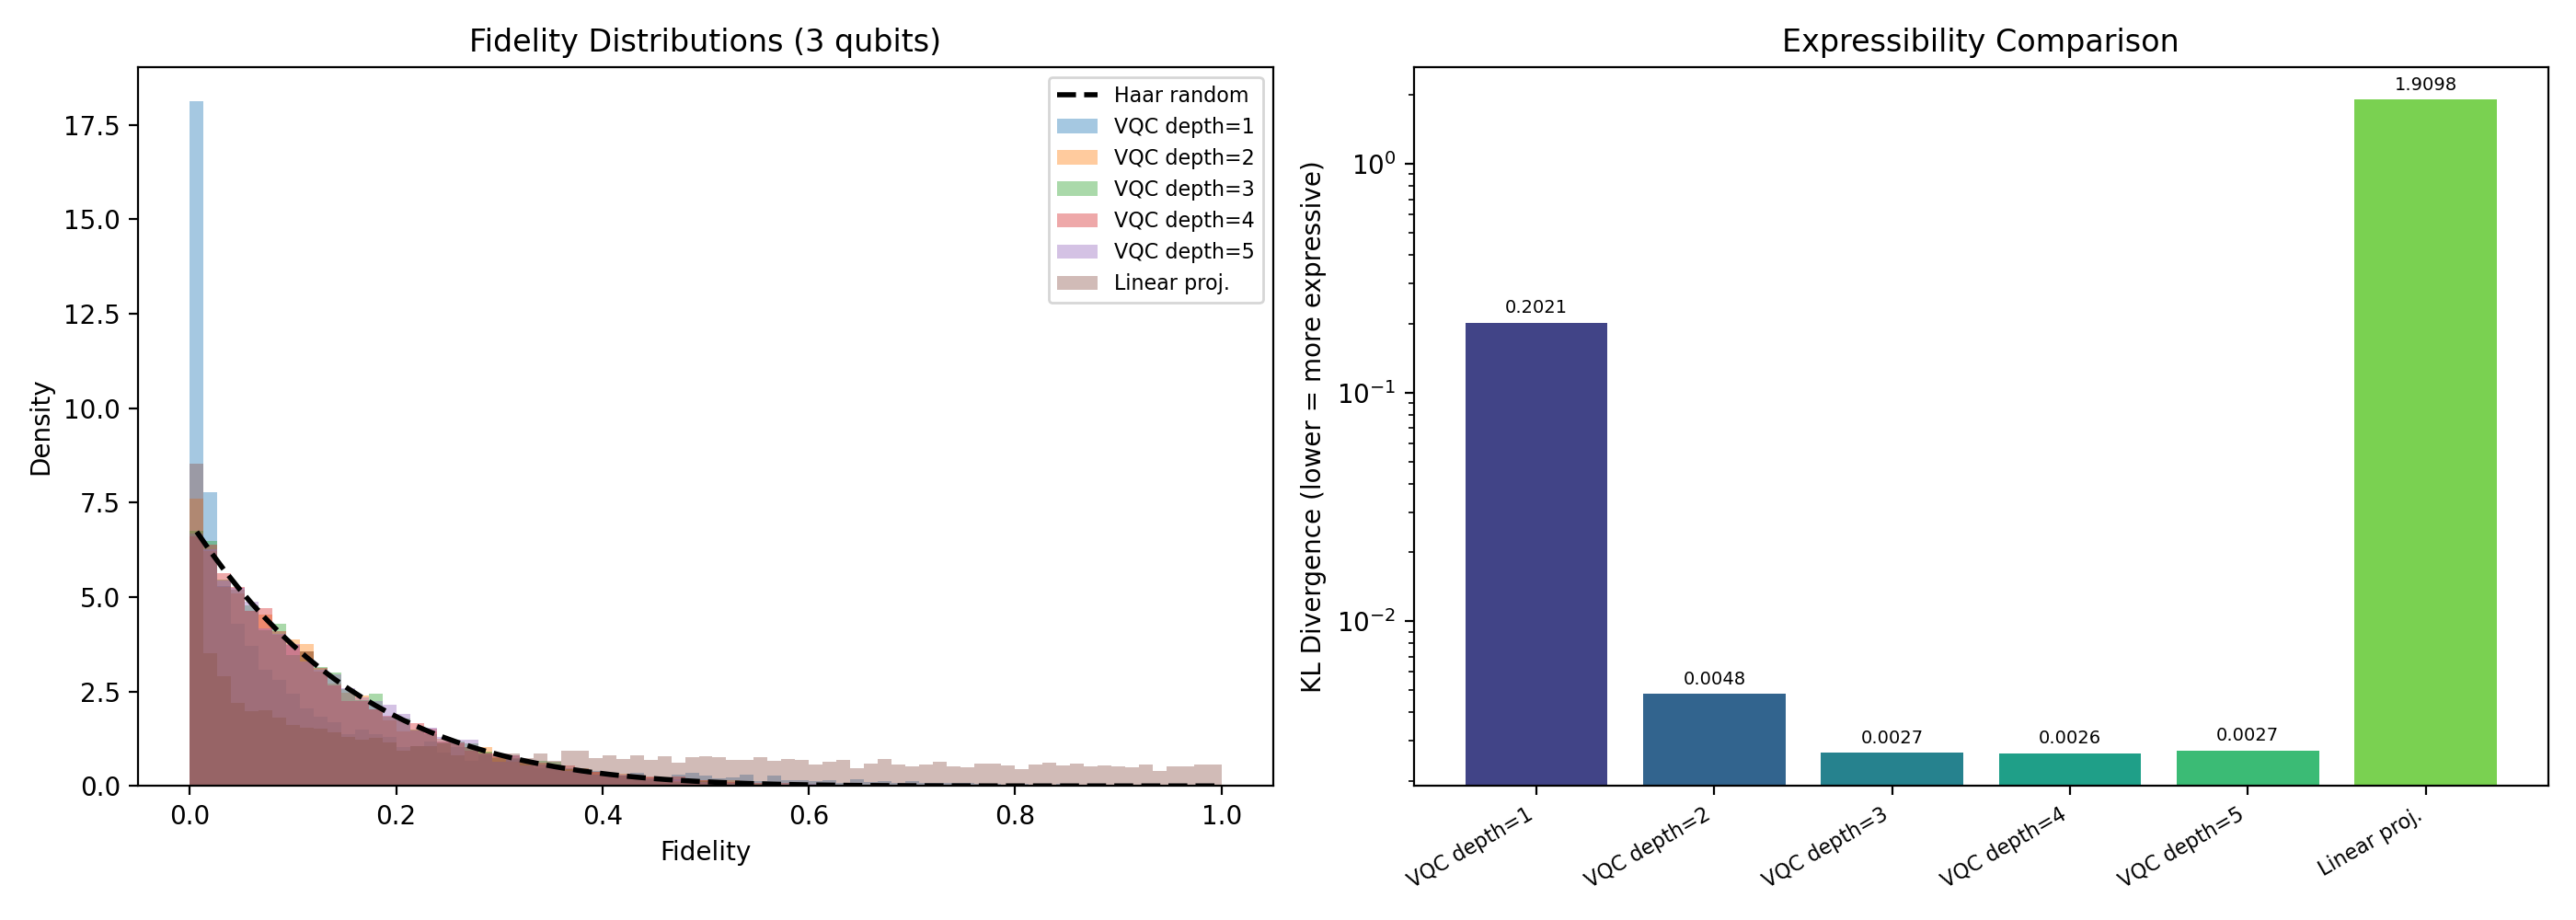
\includegraphics[width=\columnwidth]{figures/expressibility_results.png}
  \caption{Left: fidelity distributions for VQC at various depths vs.\
  Haar-random reference (dashed). Right: KL divergence (log scale).}
  \label{fig:expressibility}
\end{figure}


% =================================================================
\bibliography{references}

\end{document}
